%----------------------------------------------------------------------------
\chapter{Irodalomkutatás}
\label{sec:Search}
%----------------------------------------------------------------------------

Ebben a fejezetben bemutatom az általam használt forrásokat és technológiákat.  
Esetenként ábrákkal és kódrészletekkel illusztrálom az adott technológiát a könnyebb érthetőség kedvéért.  
Az alfejezet végén bemutatok néhány alternatív megoldást a multiplatform fejlesztésre.

\section{Felhasznált technológiák}
\label{sec:Technologies}

Ez az alfejezet a használt technológiák bemutatására fókuszál, a könnyebb érthetőség kedvéért ábrák, képek és forráshivatkozásokkal kiegészítve. 

\subsection{Jetpack Compose}
\label{sec:JetpackCompose}

A Jetpack Compose a korábbi Android fejlesztési módszer mellett hozott létre egy alternatív megoldást.  
Kezdetben nem lehetett tudni, hogyan reagálnak majd a fejlesztők az új irányra.  
Korábban a Java nyelv mellett megjelent a Kotlin nyelv is, ami később szinte teljesen leváltotta az elődjét.  
Ebből arra lehetett következtetni, hogy egy új és modernebb megoldás képes lehet felváltani az XML-alapú nézeteket.  
Jelenleg mindkét megoldás támogatott, de a fejlesztések iránya egyértelműen a Compose felé mutat.

"A Jetpack Compose egy új, deklaratív UI toolkit, amit a Google hozott létre kifejezetten natív Android alkalmazások fejlesztéséhez." \cite{GettingStartedWithJetpackCompose}  
A deklaratív nyelvekhez hasonlóan azt kell megadnunk, mit szeretnénk látni, és nem azt, hogyan történjen meg.  
Elég meghatároznunk, hogy a gomb hogyan nézzen ki, hol helyezkedjen el, és megadnunk egy lambda paraméternek, hogy a megnyomása során mi történjen.  
Mivel ez egy UI toolkit, az összes vezérlő és szerkezeti elem hasonló megjelenésű és működésű, ami egységes fejlesztői és felhasználói élményt biztosít.  
A Google ezt a Material Design keretrendszer segítségével hozta létre, amelynek újabb verzióiról itt találhatók részletes információk: \url{https://m3.material.io/}.

Az alábbiakban egy, a Google által készített rövid kódrészleten (\ref{lst:compose}.~kódrészlet) bemutatom a Compose alapjainak legfontosabb részeit. \cite{BasicCodelab}  
Az alkalmazás elkészítésének első lépése a Composable függvény megírása.  
Minden UI-t megjelenítő függvény a @Composable annotációt viseli.  
Innentől kezdve hagyományos Kotlin-függvényként viselkedik: megadhatunk tetszőleges paramétereket (például `name`, `modifier`) és alapértelmezett értékeket is.  
Egy Composable függvényből tetszőleges másik Composable függvény meghívható, amennyiben azok láthatósága megfelelő.  
Ilyen például a `Text()` függvény, amely a Material Design könyvtár egyik tagja, és egyszerű szöveget jelenít meg.

A UI megírása után azt a megfelelő helyen meg is kell jelenítenünk, erre az alkalmazás belépési pontja után van lehetőségünk.  
Android esetén ez az `Activity` `onCreate` függvénye.  
A `setContent` metódus egy lambda függvényt vár, amelyet a @Composable annotációval kell ellátni.  
Használhatjuk hozzá a Kotlin trailing lambda szintaxisát, ahol is, ha egy függvény utolsó paramétere lambda, akkor {} között megadhatjuk a függvény törzsét.  
A `BasicsCodelabTheme` is egy Composable függvény, amelyben az alapbeállítások után meghívhatjuk a saját `Greeting` függvényünket.  
A UI felépítése innentől kezdve már egyszerű. A Composable függvények megírása és egymásból való meghívása után az alkalmazás összeáll.

\begin{lstlisting}[caption={Példa a Compose használatára.}, label={lst:compose}, language=Kotlin]
    @Composable
    fun Greeting(name: String, modifier: Modifier = Modifier) {
        Text(
            text = "Hello $name!",
            modifier = modifier
        )
    }

    class MainActivity : AppCompatActivity() {
        override fun onCreate(savedInstanceState: Bundle?) {
            super.onCreate(savedInstanceState)
            setContent {
                BasicsCodelabTheme {

                Surface(
                        modifier = Modifier.fillMaxSize(),
                        color = MaterialTheme.colorScheme.background
                    ) {
                        Greeting("Android")
                    }
                }
            }
        }
    }

    // Jetpack Compose forráskód
    public fun ComponentActivity.setContent(
        parent: CompositionContext? = null,
        content: @Composable () -> Unit
    )
\end{lstlisting}

A következőkben bemutatom a UI toolkit fontosabb, általam használt részeit.  
Kitérek arra, hogy mire jók, miért ezeket választottam, és hogyan lehet őket hatékonyan alkalmazni a legújabb Compose Multiplatform verziókban.

\subsubsection{State és StateFlow}
\label{sec:State}

A State és a StateFlow hasonló problémára kínálnak megoldást.  
A State alapvetően Compose-specifikus megoldás; ha változik az értéke, akkor újracomponálás (recomposition) történik.  
Ezzel szemben a StateFlow a Kotlin nyelvben általánosan használt eszköz, amely sokkal szélesebb körű alkalmazási lehetőségeket kínál.  
Az egyszerű State-et általában egy Composable függvényen belül használják, míg a StateFlow-t inkább ViewModelekben alkalmazzák.

Ennek ellenére mindkét megoldás tökéletesen használható, és jelenleg már Compose Multiplatform alkalmazásokban is működnek.  
Mivel a ViewModel használata esetén az adatok nem vesznek el például a képernyő elforgatása során, egyszerűbb műveleteknél és adatoknál nincs lényegi különbség a két megoldás működése között.

"A StateFlow előnyei:" \cite{StateVsStateFlow}
\begin{itemize}
    \item \emph{"Flow operátorok:} A StateFlow támogat olyan operátorokat, mint a map, filter, és combine, lehetővé téve az adatok rugalmas feldolgozását és összetett adatfolyamok létrehozását."
    \item \emph{"Folyamat-megszakadás kezelése:} A SavedStateHandle-lel kombinálva biztosítja az UI állapot megőrzését, még a képernyő elforgatása vagy újraindítás esetén is."
    \item \emph{"ViewModel újrafelhasználhatóság:} A StateFlow lehetővé teszi a ViewModel függetlenítését a UI-rétegtől, ami elősegíti a moduláris, tesztelhető és újrafelhasználható architektúrát."
\end{itemize}

Az alábbi kódrészletben (\ref{lst:state}.~kódrészlet) példát találhatunk az egyszerű State használatára, amelyben például a képernyő állapotát tároljuk State-ek formájában.  
A megjelenített adatok itt a StateFlow logikáját követik.  
Létezik egy privát MutableStateFlow, amelyben az állapotváltozások történnek, például ha új adat érkezik.  
Ezen kívül van egy másik, azonos nevű érték is, amely ugyanannak a StateFlownak egy immutábilis változata. Ehhez fér hozzá a UI-réteg, így a UI közvetlenül nem módosíthatja a StateFlow-t.  
Ha módosításra van szükség, a ViewModel biztosíthat ehhez függvényeket, amelyek beállítják a privát MutableStateFlow értékét.

\begin{lstlisting}[caption={Példa a State és StateFlow használatára.}, label={lst:state}, language=Kotlin]
class TopicListViewModel: ViewModel() {
    var topicListScreenUiState: TopicListScreenUiState by mutableStateOf(TopicListScreenUiState.Loading)
    private val _topicListUiState = MutableStateFlow(TopicListUiState())
    val topicListUiState: StateFlow<TopicListUiState> = _topicListUiState
...
    fun getAllTopicList(){
        topicListScreenUiState = TopicListScreenUiState.Loading // State változás
        viewModelScope.launch {
            topicListScreenUiState = try{    // State Változás
                val result = ApiService.getAllTopicNames()
                _topicListUiState.value = TopicListUiState(     //StateFlow változás
                    topicList = result.map { nameDto ->
                        TopicRowUiState(
                            topic = nameDto.name,
                            id = nameDto.uuid
                        )
                    }
                )
                TopicListScreenUiState.Success(result) // State változás
            } catch (e: IOException) {
                TopicListScreenUiState.Error.errorMessage = e.toString()// "Network error"
                TopicListScreenUiState.Error // State változás
            }
        }
    }
}
\end{lstlisting}


\subsubsection{ViewModel}
\label{sec:ViewModel}

Az Android ViewModel már használható Kotlin- és Compose Multiplatform környezetekben is \cite{ViewModelKMP}, így természetesen ezt a jól bevált megoldást választottam.  
Egy rövid összefoglalót szeretnék adni a hivatalos dokumentáció alapján a ViewModel képességeiről \cite{ViewModelAndroid}.

A ViewModel az Android Jetpack része, és az UI állapotának megőrzésére szolgál konfigurációs változások során, például képernyőforgatáskor (\ref{fig:ViewModel}).  
Fő előnyei közé tartozik az állapot tartósítása és az üzleti logika kezelése a UI-rétegben.  
A ViewModel segít elválasztani az adatkezelést a UI-rétegtől, ehhez a ViewModelben használható a Kotlin coroutine, amely aszinkron működést tesz lehetővé.  
Ezen kívül kompatibilis olyan Jetpack könyvtárakkal, mint a Hilt, Compose, és Navigation.  
A legjobb gyakorlat szerint kerülni kell az életciklushoz kötött objektumok tárolását a ViewModelben, hogy elkerüljük a memóriaszivárgást.  

Mint minden MVI és MVVM architektúrában, az adatok elérése, átalakítása a UI számára és tartós tárolása a ViewModel feladata.  
Több megközelítés is lehetséges: minden képernyő kapjon saját ViewModelt, vagy egyetlen ViewModel legyen újrahasználva több képernyőn.  
Én az első megoldást választottam, mert így könnyebb kezelni a különböző képernyők állapotait, és egyszerűbb átlátni az egyes modulokat.

\begin{figure}[!ht]
    \centering
    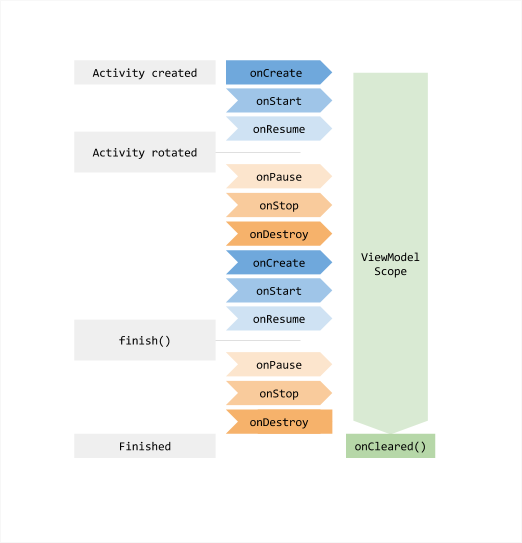
\includegraphics[width=130mm, keepaspectratio]{figures/viewmodel-lifecycle.png}
    \caption{A ViewModel általában hosszabb életű, mint egy View. Ez különösen igaz Android környezetben, ahol számolni kell a képernyő elforgatásával és az alkalmazás háttérbe kerülésével. A tartósan tárolni kívánt adatokat ezért mindig ViewModel-ben kell tárolni. \cite{ViewModelAndroid}}
    \label{fig:ViewModel}
\end{figure}

\pagebreak

\subsubsection{Navigation and routing}
\label{sec:Navigation}

Az Androidban már jól működő, navigációért felelős könyvtárak Kotlin Multiplatform fejlesztéshez is használhatóak \cite{NavigationKMP}.  
Ennek mindössze néhány egyszerű lépése van, így könnyen alkalmazható és rugalmasan működik minden környezetben.  
Az alábbi kódrészletben (\ref{lst:nav}.~kódrészlet) bemutatom a folyamatot.  
A szükséges lépések a következők \cite{NavigationKMP}:  

\begin{enumerate}
    \item Sorold fel a navigációs gráfban szereplő útvonalakat; mindegyik útvonalat egyedi string azonosít.
    \item Hozz létre egy \texttt{NavHostController} példányt, amely a navigáció kezeléséért felel.
    \item Adj hozzá egy \texttt{NavHost} komponenst az alkalmazásodhoz:
        \begin{itemize}
            \item Válaszd ki a kezdő útvonalat a korábban definiált útvonalak közül.
            \item Hozd létre a navigációs gráfot közvetlenül a \texttt{NavHost} komponensen belül, vagy programozottan a \texttt{NavController.createGraph()} függvénnyel.
        \end{itemize}
\end{enumerate}

\begin{lstlisting}[caption={Példa a Navigation használatára.}, label={lst:nav}, language=Kotlin]

//Első lépés: útvonalak létrehozása
//Érdemes sealed classt használni és data objectként létrehozni a routeokat
sealed class ExamDestination(val route: String) {
    //Lehet egyszerű
    data object LoginScreenDestination : ExamDestination("LoginScreen")
    //Vagy paraméterekkel és adatokkal ellátott
    data object TopicDetailsDestination : ExamDestination("TopicDetails") {
        const val topicIdArg = "0"
        val routeWithArgs = "$route/{$topicIdArg}"
}}

//Második lépés: NavController létrehozása
fun NavigationComponent() {
    MaterialTheme {
        val navController = rememberNavController() //Itt történik
        Scaffold() { innerPadding ->
            ExamNavHost(    //Paraméternek egy Composable függvényt vár, ezen belül is egy NavHost függvényt
                navController = navController,
                modifier = Modifier.padding(innerPadding)
            )
}}}

//Harmadik lépés: NavHost komponens hozzáadása
actual fun ExamNavHost(
    navController: NavHostController,
    modifier: Modifier
) {
    NavHost(
        navController = navController,  //NavController hozzárendelése
        startDestination = ExamDestination.MainScreenDestination.route, //Kezdő útvonal beállítása
        modifier = modifier
    ) {
        composable(        //Navigácós gráf egy elemének létrehozása
            route = ExamDestination.TopicListDestination.route,
        ) {
            TopicListScreen(
                addNewTopic = { navController.navigate(ExamDestination.NewTopicDestination.route) },
                navigateToTopicDetails = { topicId ->
                    navController.navigate("${ExamDestination.TopicDetailsDestination.route}/${topicId}")
                },
                navigateBack = { navController.popBackStack() }
            )
}}}
\end{lstlisting}
\subsection{Ktor}
\label{sec:Ktor}

A Ktor egy Kotlin-alapú HTTP-kommunikációt megvalósító könyvtár\cite{Ktor}. Alkalmas mind szerver oldali kód írására – például a REST API-m is ezt használja –, mind kliens oldali kód megvalósítására.  
A használata rendkívül egyszerű és testreszabható.  

Én egy Kotlin \texttt{object}-et használtam, amely magában foglalja az \texttt{ApiService}-et.  
Először létre kellett hozni egy HTTP-klienst, majd beállítani az alap URL-t és a tartalomtípusnak a JSON üzenetformátumot.  
Ezt követően már csak a végpont-hívásokat kellett létrehozni.

\begin{lstlisting}[caption={Példa a Ktor használatára.}, label={lst:ktor}, language=Kotlin]
object ApiService {
    private var authToken: String? = null  // Mutable token that can be updated at runtime

    private val httpClient = HttpClient() {
        install(ContentNegotiation) {   // content type beállítása
            json(Json {
                ignoreUnknownKeys = true
                prettyPrint = true
            })
        }

        defaultRequest {    // Base url beálítása
            url("http://mlaci.sch.bme.hu:46258")  // Set the base URL
            authToken?.let { token ->
                header(HttpHeaders.Authorization, "Bearer $token")  // Add the Bearer token if it's not null
            }
        }
    }
    suspend fun getAllPoints(): List<PointDto> = httpClient.get("/point").body()    //végpontok
}
\end{lstlisting}

\subsection{KotlinX-szerializáció}
\label{sec:KotlinX}

A szerializációra a JSON formátum konvertálására van szükség. Az alábbiakban a hivatalos dokumentációból olvasható egy részlet, amely jól összefoglalja a használatát.  
Ez a technológia Kotlin Multiplatform környezetben is használható.

"A szerializáció során az alkalmazások adatait egy olyan formátumba alakítjuk, amely hálózaton átvihető vagy tárolható adatbázisban vagy fájlban. Az ellenkező folyamat, a deszerializáció, az adatokat külső forrásból olvassa be és konvertálja futásidejű objektummá. A Kotlinban a szerializációhoz elérhető a kotlinx.serialization eszköz, amely Gradle bővítményt, futásidejű könyvtárakat és fordítói bővítményeket tartalmaz, így segítve a különböző nyelvű rendszerek közötti adatcserét, mint a JSON és a protocol buffers formátumokkal."\cite{Serialization}

\subsection{CameraX}

A CameraX technológia kizárólag Android platformon használható.  
Itt azonban egy nagyon széles és gazdag API-t biztosít a fejlesztéshez.  
A legfontosabb felhasználható funkciói a Preview, azaz előnézet, amikor kép készítése nélkül megjelenik a képernyőn a kamera képe, valamint az Image Analysis, azaz képfeldolgozó funkcionalitás.  
Hozzáférhetünk a buffer tartalmához, így felhasználhatjuk azt különböző algoritmusok futtatásához, vagy összekapcsolhatjuk a Google ML-Kit technológiákkal (\refstruc{sec:MLKit}).  
A képeket menteni is tudjuk, hasonlóan a beépített kamera alkalmazáshoz, és ugyanúgy videót is rögzíthetünk vele.  
Ez a leírás a Google Android Developers dokumentációja alapján készült. Részletesebb információk itt találhatók: \cite{CameraX}

\subsection{ML-Kit}
\label{sec:MLKit}

Az ML-Kit a Google által fejlesztett mesterséges intelligencia alapú API.  
Számtalan felhasználási területtel rendelkezik, ezek közül néhányat felsorolok: szöveg- és arcfelismerés, dokumentum szkennelés, kép feliratozás, fordítás, nyelv detekció és még számos más lehetőség.  
Én ezek közül az Androidos alkalmazásban a képen történő szövegfelismerést próbáltam ki \cite{MLKit}.  
Sajnos ez a funkció is Android-specifikus, így egy iOS alkalmazásban ez a probléma más megközelítést igényelne.  
Ez a technológia még messze nem tökéletes, de kipróbálásra mindenképpen érdekes és hasznos lehet.

\subsection{Accompanist-engedélykezelés}

Az engedélykezelés nem egyszerű feladat az Android rendszerekben, ezért célszerű erre kifejlesztett könyvtárakat használni.  
Egy ilyen könyvtár az Accompanist, amelyet a Google fejlesztett.  
A használata jelentősen leegyszerűsíti ezt a bonyolult folyamatot, néhány egyszerű lépéssel egy kész megoldást kapunk.

Elsőként a szükséges engedélyeket be kell jegyezni a manifest fájlba.  
Következő lépésként ellenőrizni kell, hogy az alkalmazás rendelkezik-e a szükséges engedélyekkel vagy sem.  
Amennyiben nem, akkor a használat előtt ezt kérnünk kell, de ezt csak úgy tehetjük meg, hogy a többi funkció elérhető legyen.  
Az én esetemben csak a szövegfelismerő funkcióra kattintás után kérem el az engedélyt, de maga a válaszokat elküldő képernyő használható az engedélyek nélkül is.  

Az elkért engedélyeket egy \texttt{permissionState}-ben tároljuk, így innen ellenőrizhető, hogy korábban a felhasználó már megadta-e őket.  
Egyedül a veszélyes engedélyeket kell ilyen módon elkérni, mint például a kamera használata.  
Nem veszélyes engedélyek, például az internet hozzáférés, egyszerűen a manifest fájlban rögzíthetők \cite{Permissions}.

\subsection{PdfDocument és PDFBox}

A PdfDocument a Google által fejlesztett PDF-szerkesztő eszköz.  
Segítségével egy PDF fájlba tetszőlegesen elhelyezett szöveget és képeket írhatunk.  
Létrehozhatók különböző \texttt{Paint} objektumok, amelyekkel egyszerűen rajzolhatók táblázatok, és formázható a szöveg.  
Ez a megoldás csak Android eszközökkel kompatibilis.

"Az Apache PDFBox® könyvtár egy nyílt forráskódú Java eszköz PDF dokumentumok kezelésére. Lehetővé teszi új PDF dokumentumok létrehozását, meglévő dokumentumok módosítását, és tartalom kinyerését a PDF fájlokból. Az Apache PDFBox több parancssori eszközt is tartalmaz, és az Apache License v2.0 alatt került kiadásra." \cite{PDFbox}  

Hasonlóan használható, mint a PdfDocument, de az API készletük némileg eltér.  
Bár az Androidra kifejlesztett exportálás funkció korábban elkészült, egy multiplatform rendszerben a PDFBox megoldást javasolnám minden platformon, hogy konzisztens eredményeket érjünk el.

\subsection{Kotlin- és Compose Multiplatform}
\label{sec:KCMP}

Többször beszéltem már a Kotlin Multiplatform és a Compose Multiplatform fogalmakról.  
Legkönnyebben úgy lehet leírni a kapcsolatukat, mint a Compose Multiplatform részhalmazát a Kotlin Multiplatformnak.  
Számos nagy cég használja a KMP technológiát, köztük a Netflix, a 9GAG, a McDonald's és a Philips \cite{KotlinMultiplatformStable}.  

Az általam korábban felsorolt technológiák közül, amelyek leginkább ebbe a kategóriába esnek, a Ktor (\refstruc{sec:Ktor}) és a KotlinX szerializáció (\refstruc{sec:KotlinX}).  
Mivel 2024 őszén elérhetővé vált az Android ViewModel (\refstruc{sec:ViewModel}) és a navigáció (\refstruc{sec:Navigation}) is, ezek is ide sorolhatók már a state-ekkel együtt (\refstruc{sec:State}).  

Az egyetlen fontosabb rész, amit kihagytam, az maga a Compose deklaratív UI toolkit (\refstruc{sec:JetpackCompose}), amely a Compose Multiplatform alapját képezi.  
2021-ben vált lehetővé a Compose használata nem csak Android alapú rendszerekhez, míg a KMP 2017-ben kezdte meg az útját.  
Nagy jelentősége van a CMP-nek, mivel így kizárólag Kotlin nyelven Android fejlesztők tudnak iOS és asztali alkalmazást fejleszteni minimális natív kóddal, de mégis natív élményt nyújtva.  
Jelenleg a webes irány még alpha verzióban van, de jelenleg is folyik a fejlesztés a Kotlin WASM-re (WebAssembly) való hatékony fordításán. A Kotlint JavaScript kóddá is le lehet fordítani, a Java mellett.  

Háromféle módon lehet Kotlin Multiplatform kódbázist fejleszteni (\refstruc{fig:KMPTypes}).  
Az első, bal oldali ábra értelmezése szerint a kódbázis egy kis része íródik KMP-ben, például csak az adatbázis vagy REST API elérés.  
A következő ábra azt mutatja, hogy a logika teljes egészében KMP-ben íródik, így például használják a ViewModeleket (\refstruc{sec:ViewModel}), de a UI natív módon készül: Androidra Compose-ban, iOS-re SwiftUI-ban.  
Az utolsó ábra már a Compose Multiplatform megjelenése, amikor minden platformra Compose-ban készül el a felhasználói felület.  
Balról jobbra haladva egyre nő a kód újrafelhasználhatósága, így kevesebb munka szükséges, és könnyebb is a kód karbantartása, mivel előreláthatólag egyre kevesebb helyen kell módosítani azt.

\begin{figure}[!ht]
    \centering
    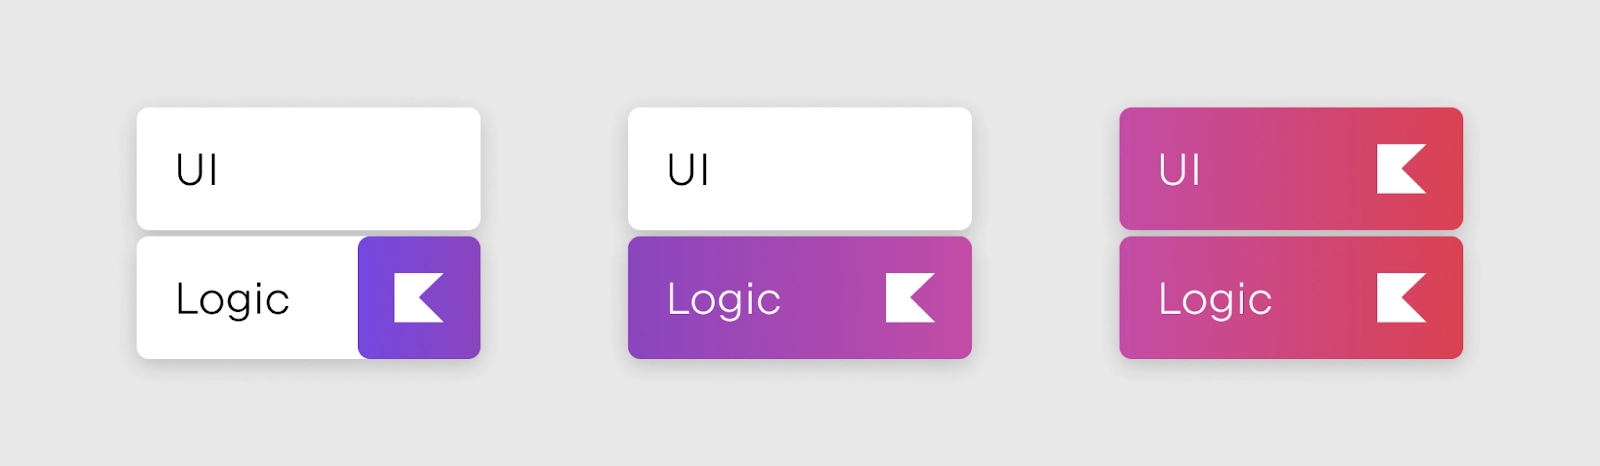
\includegraphics[width=150mm, keepaspectratio]{figures/KMP-types.png}
    \caption{A KMP fejlesztés változatai. \cite{KotlinMultiplatformStable}}
    \label{fig:KMPTypes}
\end{figure}

Semmi sem teljesen tökéletes, így előfordulhat, hogy az egyik platformon máshogy nem lehet vagy nem érdemes valamit megvalósítani, mint például egy asztali alkalmazáson egy fotó elkészítését az én példámban.  
Ilyenkor jöhetnek szóba az \texttt{expect} és \texttt{actual} függvények. A közös kódban ilyenkor egy függvénytörzset definiálunk, és csak itt lehet alapértelmezett paramétereket beállítani, például egy \texttt{Modifier}-t egy \texttt{Composable} függvény esetén.  
A megvalósítás ilyenkor az alkalmazás-specifikus kódban történik (\texttt{androidMain}, \texttt{desktopMain}, \texttt{iOSMain}) (\ref{lst:ExpectActual}.~kódrészlet).  
Ehhez az \texttt{actual} függvényt kell megvalósítani, és a platformtól függően ezek fognak automatikusan meghívódni, mivel a build során ezek kerülnek behelyettesítésre az \texttt{expect} függvény helyére.  
Már léteznek \texttt{actual} és \texttt{expect} osztályok is, amelyeket én alkalmaztam, de ez még kísérleti verzióban van.

\begin{lstlisting}[caption={Expect és actual használata}, label={lst:ExpectActual}, language=Kotlin]
//commonMain-ben lévő expect függvénytörzs, alapértelmezett paraméterrel.
@Composable
expect fun MainCameraScreen(examId: String = "0", navigateBack: () -> Unit)

//androidMain-ben lévő valós megvalósítás
@Composable
actual fun MainCameraScreen(examId: String, navigateBack: () -> Unit) {

    val cameraPermissionState: PermissionState = rememberPermissionState(android.Manifest.permission.CAMERA)

    MainCameraContent(
        hasPermission = cameraPermissionState.status.isGranted,
        examId = examId,
        onRequestPermission = cameraPermissionState::launchPermissionRequest,
        navigateBack = navigateBack
    )
}

//desktopMain-ben lévő placeholder megvalósítás, értesíti a felhasználót, hogy ez a funkció az eszközén nem támogatott
@Composable
actual fun MainCameraScreen(examId: String, navigateBack: () -> Unit) {
    Scaffold(
        topBar = {
            TopAppBarContent(stringResource(Res.string.camera), navigateBack)
        },
        content = { innerPadding ->
            UnsupportedFeatureScreen(modifier = Modifier.padding(innerPadding))
        }
    )
}
\end{lstlisting}

\subsection{Gradle build rendszer}

A Compose Multiplatform projektek is a Gradle build rendszert használják, elsősorban a függőségek megszerzésére és az alkalmazás létrehozására.  
Egy átlagos fejlesztőnek mindössze annyi a dolga, hogy kigyűjti a használt függőségeket, és a fejlesztőkörnyezet általában segít a megfelelő verziók megtalálásában.  
Újabban a Kotlin DSL használata terjedt el.

"A DSL (Domain-Specific Language) egy programozási nyelv, amely egy meghatározott problémakör megoldására összpontosít. Az általános célú nyelvektől eltérően a DSL-ek, például az SQL és a regexek, csak egy szűk területre fókuszálnak, ami lehetővé teszi a problémák deklaratív módon való megoldását."\cite{KotlinDSL}  
Ennek segítségével egyszerűbben adhatjuk meg a Gradle-függőségeket (\ref{lst:KotlinDSL}.~kódrészlet).

\begin{lstlisting}[caption={Kotlin DSL}, label={lst:KotlinDSL}, language=Kotlin]
kotlin {    //Részlet a build.gradle fájlból
    androidTarget {
        compilerOptions {
            jvmTarget.set(JvmTarget.JVM_11)
        }
    }
    sourceSets {
        androidMain.dependencies {
            implementation(libs.androidx.activity.compose)
        }
    }
}
\end{lstlisting}

Ezen kívül a verziók egyszerűbb karbantartására használhatunk egy version catalog fájlt, ez a \texttt{libs.version.toml}.  
A TOML a "Tom's Obvious, Minimal Language" rövidítése, és elsősorban egyszerűbb konfigurációs fájlok esetében használják; egyfajta "butább" YAML-formátum.  
A szükséges részei a \texttt{[versions]} és a \texttt{[libraries]}, illetve szükség lehet a \texttt{[plugins]}-re is (\ref{lst:toml}.~kódrészlet). Az itt megadott értékekre lehet hivatkozni a \texttt{build.gradle} fájl(ok)ban.

\begin{lstlisting}[caption={Version catalog}, label={lst:toml}, language=Kotlin]
#Részlet a libs.version.toml fájlból

[versions]
agp = "8.2.2"
android-compileSdk = "34"
android-minSdk = "24"
android-targetSdk = "34"
androidx-activityCompose = "1.9.2"
androidx-appcompat = "1.7.0"
androidx-constraintlayout = "2.1.4"
androidx-core-ktx = "1.13.1"

[libraries]
androidx-core = { module = "androidx.core:core", version.ref = "androidx-core-ktx" }
androidx-core-ktx-v1120 = { module = "androidx.core:core-ktx", version.ref = "coreKtx" }

[plugins]
androidApplication = { id = "com.android.application", version.ref = "agp" }
androidLibrary = { id = "com.android.library", version.ref = "agp" }
\end{lstlisting}

\subsection{Fejlesztőkörnyezetek}

Fejlesztőkörnyezetként a JetBrains egyik eszközét, a Fleet-et választottam.  
Ezt kifejezetten multiplatform fejlesztéshez készítették, és támogatja azokat a nyelveket, amelyek ebben a témában szóba jöhetnek.  
Minden funkcióval rendelkezik, amit a JetBrains natív fejlesztésre készült IDE-i is nyújtanak, például kódkiegészítéssel és kódkiemeléssel, így nem kell IDE-t váltani, ha éppen más nyelven kell dolgozni.

"Amikor az Smart Mode engedélyezve van, a Fleet nyelvspecifikus funkciókat kínál, mint például a kódkiegészítés, navigáció, hibakeresés és refaktorálás. Ha ez a mód le van tiltva, a Fleet egyszerű szövegszerkesztőként működik; gyorsan meg lehet nyitni fájlokat és módosításokat végezni, de a fejlettebb funkciók nélkül. A háttérben a Fleet kiválasztja a kód feldolgozásához szükséges háttérmotort. Intelligens módban például a Kotlin feldolgozási motorja az IntelliJ IDEA-hoz használt motor, így ismerős funkciók maradnak elérhetők." \cite{Fleet}

Egy másik hasznos funkció, hogy egy helyről lehet minden platformra buildelni az alkalmazást (\refstruc{fig:RunConfigs}), így nem kell egy külön Android Studio-t és Xcode-ot is megnyitni, ha szeretnéd tesztelni az alkalmazást az adott eszközön.

A fő fejlesztőkörnyezeten kívül, amíg csak az Android applikációt fejlesztettem, az Android Studio-t használtam.  
A REST API fejlesztéséhez és karbantartásához szintén a JetBrains termékét, az IntelliJ IDEA Ultimate-et használtam, amely kifejezetten Java és Kotlin projektekhez készült.  
Kisebb mértékben a fejlesztéshez, és nagyobb mértékben a dokumentációhoz és a szakdolgozat megírásához a Visual Studio Code-ot használtam, mivel sok hasznos bővítménnyel rendelkezik, például \LaTeX és PlantUML használatához.

\begin{figure}[!ht]
    \centering
    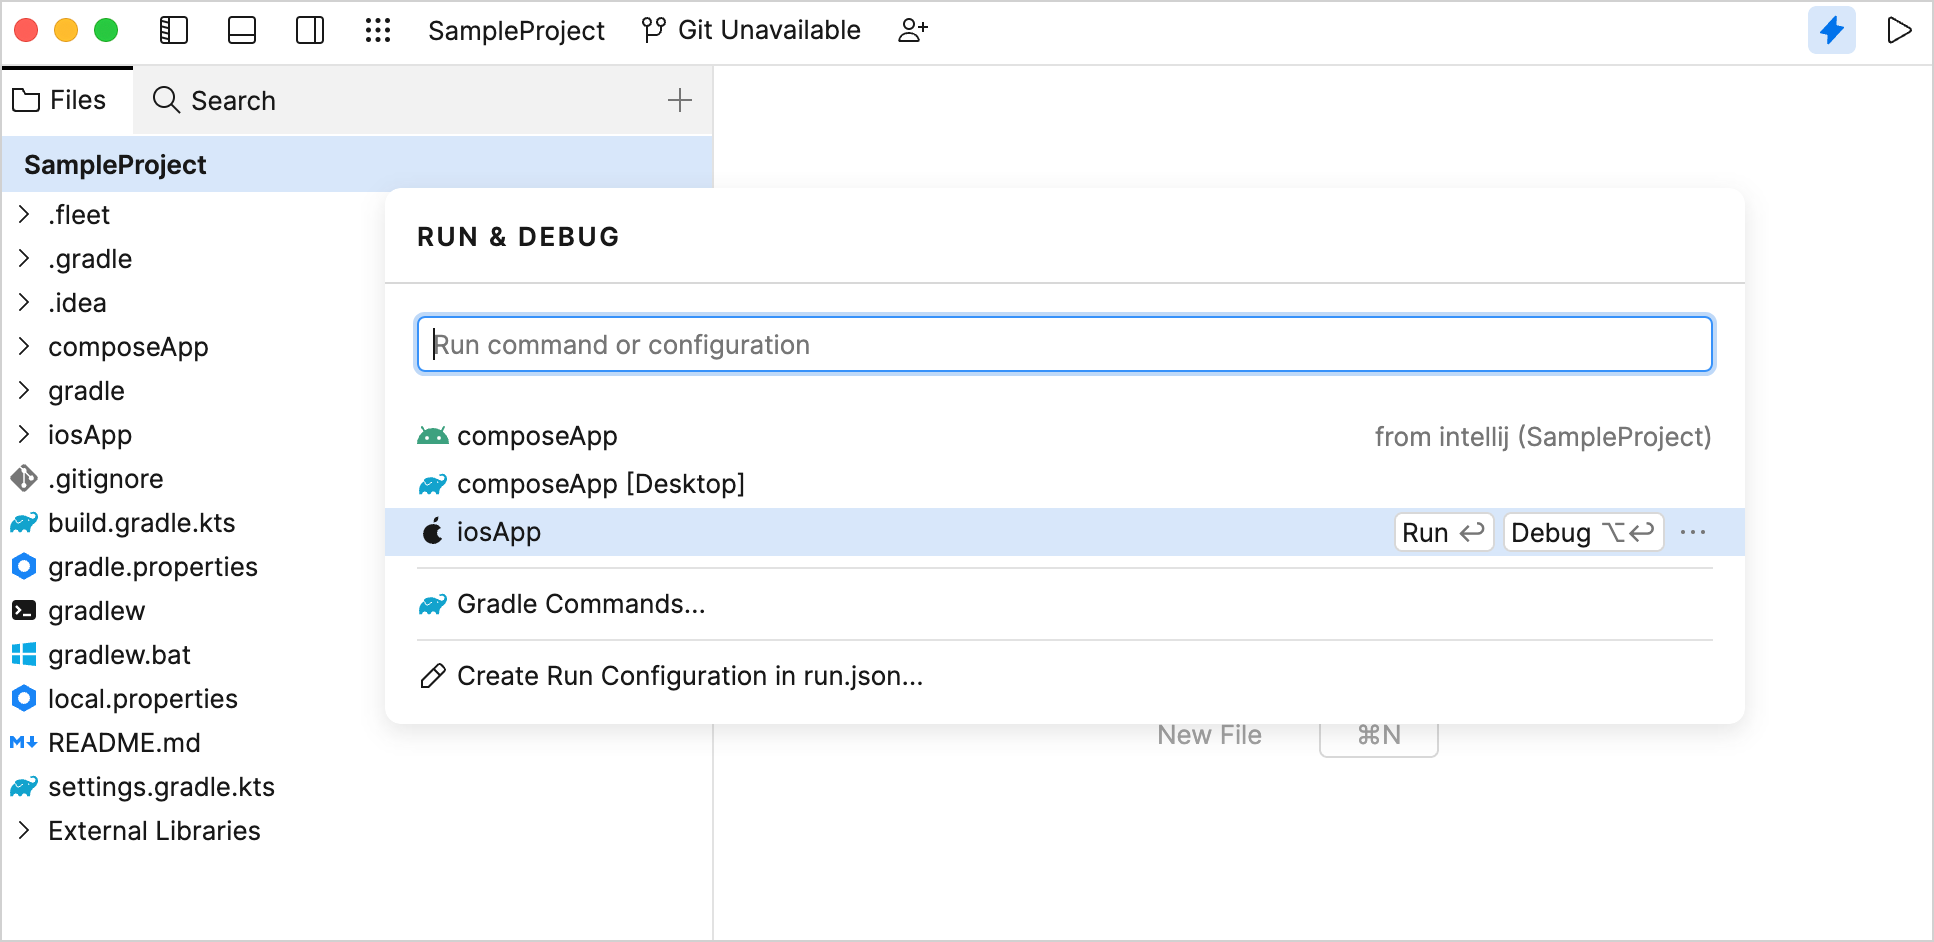
\includegraphics[width=150mm, keepaspectratio]{figures/fleet-run-configurations.png}
    \caption{A különböző eszközökre egy helyen lehet buildelni és futtatni az alkalmazást. \cite{Fleet}}
    \label{fig:RunConfigs}
\end{figure}


\subsection{REST API, Postman és adatbázis}

A kliens oldali alkalmazásokat egy saját REST API szolgálja ki.  
Ezt az előző félévben készítettem el, teljes egészében Kotlin nyelv felhasználásával. A HTTP kommunikáció megvalósításához a már korábban \refstruc{sec:Ktor}-ban bemutatott Ktor-t használtam.  
Itt a szerver oldali funkcionalitás került előtérbe. A szerializáció itt is a \refstruc{sec:KotlinX}-ban leírtak szerint történt.  
Az adatbázis az úgynevezett code-first felfogás alapján készült. Ez azt jelenti, hogy kódban leírtam az adatbázis felépítését, és a kigenerálását rábíztam az Exposed-ra, ami a JetBrains által fejlesztett, adatbázis-elérést lehetővé tevő könyvtár.  
A használt adatbázis a javaslatok alapján a PostgreSQL lett. Ennek a folyamatnak egy részletesebb leírása a \cite{Backend} forrásban olvasható, ez alapján készítettem el a saját szerveremet.

Mind az adatbázis, mind a REST API egy-egy Docker-konténerben fut egy virtuális gépen, így biztosítva a folyamatos elérhetőséget.  
"Mi az a Docker? A Docker egy nyílt platform alkalmazások fejlesztésére, szállítására és futtatására. Lehetővé teszi, hogy az alkalmazásokat elválasszuk az infrastruktúrától, így gyorsabban tudunk szoftvereket szállítani. A Docker segítségével az infrastruktúrát ugyanúgy kezelhetjük, mint az alkalmazásokat. A Docker szállítási, tesztelési és kódtelepítési módszertanait kihasználva jelentősen csökkenthetjük az időt a kód megírása és a termelési környezetben való futtatása között." \cite{Docker}  

"A Docker platform: A Docker lehetőséget biztosít arra, hogy az alkalmazást egy lazán izolált környezetben, úgynevezett konténerben csomagoljuk és futtassuk. Az izoláció és a biztonság lehetővé teszi, hogy egy adott gépen egyszerre több konténert futtassunk. A konténerek könnyűsúlyúak, és mindent tartalmaznak, ami szükséges az alkalmazás futtatásához, így nem kell a gazdagépre telepített környezetre támaszkodni. A konténereket megoszthatjuk munka közben, biztosítva, hogy mindenki ugyanazt a konténert kapja, amely ugyanúgy működik." \cite{Docker}

Az API saját DNS-címmel is rendelkezik, így könnyen megjegyezhető és elérhető a fejlesztés és tesztelés során is.  
A teszteléshez a Postmant használtam. Ez egy olyan alkalmazás, amiben HTTP-kéréseket lehet létrehozni, és a mezőket tetszőlegesen testreszabni.  
Gyakran volt rá szükség ebben a félévben is, mert bizonyos adatformátumok vagy követelmények változtak, és ez sokkal hatékonyabb hibakezelést tett lehetővé, mint egy böngészős HTTP-kérés vagy az alkalmazásból történő debugolás.

\subsection{Kipróbált, de végül nem használt egyéb érdekes megoldások}

Az önálló laboratórium során elkészített alkalmazás sok technológiát felhasznált, elsősorban kísérletezés miatt.  
Ezek egy részére találtam jól használható multiplatform alternatívát, más részükre nem, vagy csak nagyon sok munkával lehetett volna megvalósítani.  
Rendelkezett lokális Room-adatbázissal is; erre egy alternatív megoldás a multiplatform területen az SQLDelight technológia. 2024 őszétől azonban a Room is támogatott.  
Ezt felhasználók tárolására használtam Firebase-integrációval. A Firebase sajnos sokkal nehezebben használható ebben a környezetben, és mivel az alkalmazás jelenlegi állapotában a felhasználóknak nincs jelentősége, ezek nem kerültek be a végső alkalmazásba.

Egy korábbi multiplatform ViewModel alternatíva a moko-viewmodel (Mobile Kotlin Model-View-ViewModel architecture) volt, de ennél kényelmesebb az Androidos.  
Mivel nem volt szükség felhasználó- és login-szolgáltatásokra, illetve lokális adatbázisra, így elvetettem a dependency injection használatát. Ezért a ViewModel-ek létrehozása sem okozott akkora problémát. Az Androidban használt Hilt itt nem használható, és a Koin, ami egy hasonló multiplatform implementáció, nem könnyítette volna meg annyira a folyamatot, mint a Hilt.  
Ezeknél a függőségeknél a verziók összehangolása sem volt egyértelmű feladat. Minél több függőségre van szükség, annál nagyobb a valószínűsége, hogy valami összeütközik vagy eltörik egy új frissítés miatt, főleg, ha az nem egy hivatalos függőség a Google vagy a JetBrains által.  
Külön-külön rendesen működtek, de az előbb felsorolt problémák miatt úgy döntöttem, hogy egyszerűbb és letisztultabb megoldásokat használok a függőségek terén.

\section{Hasonló multiplatform megoldások összehasonlítása}
\label{sec:SimilarSolutions}

Négy különböző technológiát vizsgáltam meg, és korábbi tapasztalataim, illetve információim alapján próbáltam választani közülük.  
Az első a Compose Multiplatform, a második a MAUI, a harmadik a React Native, a negyedik a Flutter.  
Az alábbiakban található egy rövid összefoglalás ezekről a technológiákról.

\textbf{Kotlin és Compose Multiplatform}: A JetBrains és a Google által fejlesztett technológiák, amelyek lehetővé teszik a kód megosztását platformok között, anélkül hogy új nyelvet kellene bevezetni. Nemrégiben stabilizálták, és támogatja a felhasználói felület megosztását a Compose Multiplatform segítségével. \cite{KotlinCrossPlatformFrameworks}  

\textbf{.NET MAUI}: A Microsoft C\# és XAML alapú keretrendszere, amely cross-platform API-kat, hot reload funkciót biztosít, és asztali és mobil platformokra is céloz. \cite{KotlinCrossPlatformFrameworks}  

\textbf{React Native}: A Meta JavaScript alapú keretrendszere, amely a natív UI-t helyezi előtérbe, erős közösségi támogatással. A Fast Refresh funkciót használja, és a Flipper-t integrálja hibakereséshez. \cite{KotlinCrossPlatformFrameworks}  

\textbf{Flutter}: A Google Dart alapú keretrendszere, amely a hot reload és az egyéni renderelés révén ismert. Támogatja a Material Design-t, és széles körben használják cross-platform alkalmazásokhoz (pl. eBay, Alibaba). \cite{KotlinCrossPlatformFrameworks}  

A kiválasztás során számos szempontot figyelembe vettem. Fontos volt a tanulási lehetőség a témából, lehetőleg olyan módon, hogy azt később is tudjam kamatoztatni.  
Egy másik szempont volt, hogy ne legyen teljesen ismeretlen az használt eszköz és környezet, ennek célja az volt, hogy az időm nagy részét ne tutorial videók nézésével töltsem az alapoktól kezdve, hanem a dokumentációk alapján is el tudjak igazodni hatékonyan.  
Nem utolsó szempont volt, hogy szerettem volna folytatni az előző félévben elkezdett alkalmazásomat.  
Az összes opció megvizsgálása után alkalmasnak találtam a Compose Multiplatformot a szakdolgozat témájaként.

Ezek közül az utolsót zártam ki a leghamarabb. A fenti négy közül ez az egyetlen, amely nem natív UI élményt nyújt a felhasználóknak, és egy számomra teljesen ismeretlen Dart nyelven kell programozni. Elsősorban mobilos fejlesztésre használják, de a többi része nem optimális, én pedig ennél egy általánosabb megoldást kerestem. \cite{Flutter}  

A következő technológia, amit kizártam, a React Native volt. Ez a React egyfajta változata, amely natív élményt tud nyújtani weben, Androidon, iOS-en és asztali alkalmazásokon is.  
Ez egy JavaScript/TypeScript és HTML alapú megoldás. Korábbi tapasztalataim alapján ezek a nyelvek nem alkalmasak egy nagy méretű projekt fejlesztésére és karbantartására.  
JavaScriptben gyorsan lehet fejleszteni, de nagyon nehéz utána a kód továbbfejlesztése és karbantartása. \cite{ReactNative}  

A MAUI egy .NET alapú megoldás, így C\# nyelven lehet programozni. A UI XAML alapokon nyugszik, hasonlóan a WinUI-hoz.  
Ez a megoldás a Windowsos asztali alkalmazásokhoz hasonlít leginkább felfogásban és programozásban.  
Volt több elődje is, de jelenleg ez a legújabb változata a Windows alapokon nyugvó multiplatform fejlesztésnek.  
A legfőbb indok az elvetésére az volt, hogy én elsősorban Android-fejlesztő vagyok, és ha van lehetőség, akkor abból az irányból szerettem volna kiindulni.  
Egy másik érv ellene, hogy webes irányban nincs elmozdulás, míg az előző kettőnél igen, illetve a Compose Multiplatform is nyit ebbe az irányba. \cite{MAUI}  

Mindent összevetve a Compose Multiplatform volt számomra a legalkalmasabb és legérdekesebb technológia.  
Ebben volt a legtöbb tapasztalatom, és a későbbiekben is szeretnék ezen a területen dolgozni, akár natív Android fejlesztés, akár a Compose és Kotlin Multiplatform világában.  
Továbbá mindig érdekes kihívás egy éppen aktívan fejlődő technológiát megismerni és dolgozni benne.  
Így azt is ki tudtam próbálni, hogy milyen nehézségekkel jár egy natív alkalmazás multiplatformba való átültetése.
